\chapter{Decision Trees: Intuition and Geometry}
\label{chap:decision_tree_intuition}

\section{Introduction}
In previous chapters, we studied Linear Models (Linear Regression, Logistic Regression, SVM) which try to find a mathematical equation (a line or hyperplane) to separate data.
\textbf{Decision Trees} take a completely different approach. Instead of finding a complex formula, they ask a series of simple questions.

\begin{definition}
\textbf{Decision Tree}: A hierarchical Supervised Learning model that splits data into subsets based on the value of input features. It mimics human decision-making by asking a sequence of "if-else" questions to arrive at a prediction.
\end{definition}

\section{The Intuition: The "20 Questions" Game}
Imagine you are playing a game with a friend. You have to guess the animal they are thinking of, but you are only allowed to ask \textbf{Yes/No} questions.

\begin{itemize}
    \item \textbf{Question 1}: Is it bigger than a cat?
    \begin{itemize}
        \item \textit{Answer}: No. (You immediately rule out Elephants, Tigers, etc.)
    \end{itemize}
    \item \textbf{Question 2}: Does it fly?
    \begin{itemize}
        \item \textit{Answer}: Yes. (You assume it's a bird or insect).
    \end{itemize}
    \item \textbf{Question 3}: Is it green?
    \begin{itemize}
        \item \textit{Answer}: Yes.
    \end{itemize}
    \item \textbf{Conclusion}: It is a \textbf{Parrot}.
\end{itemize}

This is exactly how a Decision Tree works.
\begin{enumerate}
    \item The entire dataset starts at the \textbf{Root Node}.
    \item The algorithm picks the "Question" (Feature) that divides the data most effectively.
    \item It repeats this process until it reaches a conclusion (\textbf{Leaf Node}).
\end{enumerate}

\section{Geometric Intuition: Space Cutting}
To understand Decision Trees mathematically, we must view them as \textbf{Space Cutters}.
\begin{itemize}
    \item Review: \textbf{Linear Regression} draws a single diagonal line: $y = mx + c$.
    \item **Decision Trees** cannot draw diagonals. They draw \textbf{Orthogonal Cuts} (lines parallel to the X or Y axes).
\end{itemize}

\begin{itemize}
    \item If the rule is $X < 5$, it draws a vertical line at $X=5$.
    \item If the next rule is $Y < 3$, it draws a horizontal line at $Y=3$ \textit{within that region}.
\end{itemize}

By making these repeated vertical and horizontal cuts, the Tree divides the entire N-dimensional feature space into rectangular regions called \textbf{Hyper-cuboids}.

\begin{figure}[htbp]
\centering
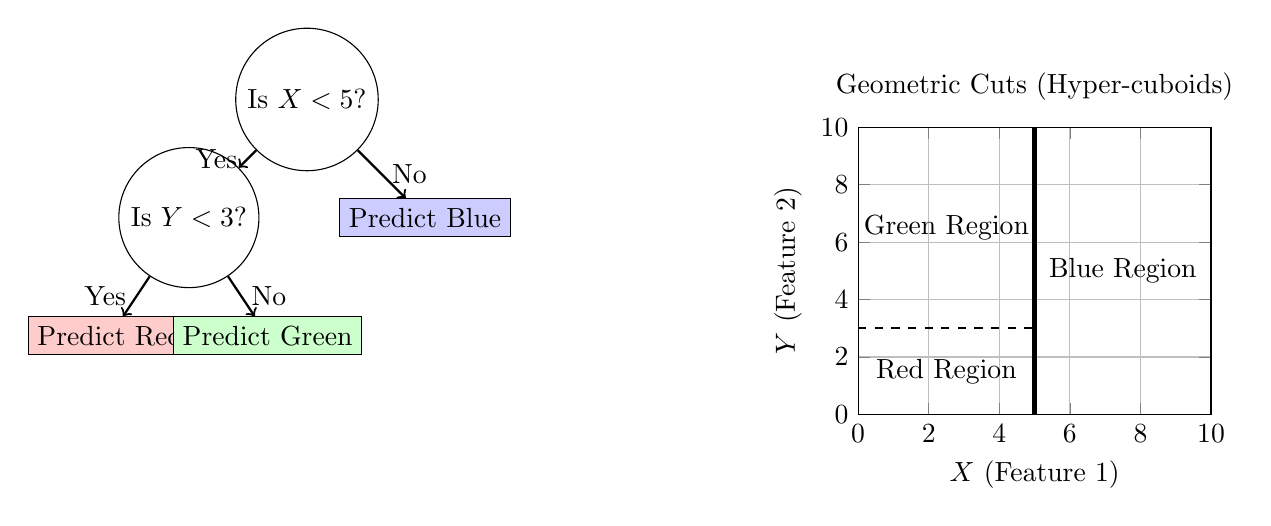
\begin{tikzpicture}
    % Tree Structure (Left)
    \node (root) at (-4, 2) [circle, draw, align=center] {Is $X < 5$?};
    \node (node1) at (-5.5, 0.5) [circle, draw, align=center] {Is $Y < 3$?};
    \node (leaf1) at (-2.5, 0.5) [rectangle, draw, fill=blue!20, minimum width=1.5cm] {Predict Blue};
    \node (leaf2) at (-6.5, -1) [rectangle, draw, fill=red!20, minimum width=1.5cm] {Predict Red};
    \node (leaf3) at (-4.5, -1) [rectangle, draw, fill=green!20, minimum width=1.5cm] {Predict Green};
    
    \draw[->, thick] (root) -- node[left] {Yes} (node1);
    \draw[->, thick] (root) -- node[right] {No} (leaf1);
    \draw[->, thick] (node1) -- node[left] {Yes} (leaf2);
    \draw[->, thick] (node1) -- node[right] {No} (leaf3);
    
    % Geometric Space (Right)
    \begin{axis}[
        at={(3cm,-2cm)},
        width=0.5\textwidth,
        xmin=0, xmax=10, ymin=0, ymax=10,
        xlabel=$X$ (Feature 1), ylabel=$Y$ (Feature 2),
        title={Geometric Cuts (Hyper-cuboids)},
        grid=major
    ]
        % Vertical Cut X=5
        \draw[ultra thick] (axis cs:5, 0) -- (axis cs:5, 10);
        \node at (axis cs:7.5, 5) {Blue Region};
        
        % Horizontal Cut Y=3 (Only where X < 5)
        \draw[thick, dashed] (axis cs:0, 3) -- (axis cs:5, 3);
        
        \node at (axis cs:2.5, 1.5) {Red Region};
        \node at (axis cs:2.5, 6.5) {Green Region};
    \end{axis}
\end{tikzpicture}
\caption{Left: The Logic flow (Tree). Right: The Geometry showing how logic converts to rectangular regions.}
\label{fig:tree_geometry}
\end{figure}

\section{Terminology}
Let us formalize the parts of a tree:
\begin{enumerate}
    \item \textbf{Root Node}: The top-most node. It contains the entire dataset ($100\%$ of samples) before any splitting happens.
    \item \textbf{Decision Node} (Internal Node): A node that splits the data further based on a condition.
    \item \textbf{Leaf Node} (Terminal Node): A node that does not split. It contains the final prediction (e.g., "This is a Cat").
    \item \textbf{Splitting}: The process of dividing a node into two or more sub-nodes.
    \item \textbf{Pruning}: The process of removing branches to reduce the size of the decision tree and prevent Overfitting.
\end{enumerate}

\section{Implementation in Python}
\begin{lstlisting}[language=Python, caption=Basic Decision Tree Classifier]
from sklearn.datasets import load_iris
from sklearn.tree import DecisionTreeClassifier, plot_tree
from sklearn.model_selection import train_test_split
import matplotlib.pyplot as plt

# Load Data
X, y = load_iris(return_X_y=True)
X_train, X_test, y_train, y_test = train_test_split(X, y, test_size=0.2)

# Train Decision Tree
tree = DecisionTreeClassifier(max_depth=3, random_state=42)
tree.fit(X_train, y_train)

# Visualize the Tree
plt.figure(figsize=(12, 8))
plot_tree(tree, filled=True, feature_names=load_iris().feature_names)
plt.title("Decision Tree Visualization")
plt.show()

print(f"Accuracy: {tree.score(X_test, y_test):.2f}")
\end{lstlisting}

\section{HOTS: Interview Questions}
\textbf{Q1: Can Decision Trees draw diagonal decision boundaries?}
\begin{itemize}
    \item No. By design, they only make cuts parallel to the axes (orthogonal cuts). To approximate a diagonal, they would need many staircase-like splits.
\end{itemize}

\textbf{Q2: Why are Decision Trees called ``Greedy'' algorithms?}
\begin{itemize}
    \item At each node, the tree picks the \textit{locally} best split (maximum Information Gain). It does not look ahead to see if a different split would be globally better. This makes it fast but potentially suboptimal.
\end{itemize}

% ========================================
% SECTION: QUICK REFERENCE
% ========================================
\section{Quick Reference Card}

\begin{center}
\fbox{\parbox{0.9\textwidth}{
\textbf{DECISION TREES - CHEAT SHEET}
\vspace{0.3cm}

\textbf{Core Idea}: Game of ``20 Questions'' - split data with yes/no questions

\textbf{Geometry}: Orthogonal cuts create axis-parallel hyper-cuboid regions

\textbf{Key Terminology}:
\begin{itemize}
    \item \textbf{Root}: First decision node
    \item \textbf{Leaf}: Terminal node with prediction
    \item \textbf{Depth}: Longest path from root to leaf
\end{itemize}

\textbf{Splitting Criteria}:
\begin{itemize}
    \item Classification: Entropy, Gini Impurity
    \item Regression: Variance Reduction (MSE)
\end{itemize}

\textbf{Sklearn}: \texttt{DecisionTreeClassifier(max\_depth=5)}

\textbf{Interview Gold}:
\begin{itemize}
    \item Greedy: picks locally best split (not globally optimal)
    \item Cannot draw diagonal boundaries (only orthogonal)
    \item No scaling needed! (based on thresholds, not distances)
\end{itemize}
}}
